%%%%%%%%%%%%%%%%%%%%%%%%%%%%%%%%%%%%%%%%%%%%%%%%%%%%%%%%%%%%%%%%%%%%%%%%%%%%%%%%%%%%%%%%%%%%%%%%%%%
% Chapter 3 -> Methods
% Author: Mingbo Cheng
%%%%%%%%%%%%%%%%%%%%%%%%%%%%%%%%%%%%%%%%%%%%%%%%%%%%%%%%%%%%%%%%%%%%%%%%%%%%%%%%%%%%%%%%%%%%%%%%%%%
\addbibresource{~/MEGA/MEGAsync/phd/thesis_Cheng/preamble/thesis.bib}
\chapter{Methods}
\label{chapter:methods}
\graphicspath{{chapter3/figs}}

In the previous chapter, we introduced the concept of profiling the single-cell transcriptome, genome, epigenome, and proteome, along with simultaneous sequencing. We also outlined the common workflow for analyzing single-cell sequencing data from different protocols and that of single-cell multimodal analysis. We discussed the challenges associated with single-cell multimodal integration due to various feature distributions and types. To tackle this, our goal is to develop computational methods to effectively integrate single cells of multiple modalities. Another challenge in single-cell multimodal analysis is inferring a trajectory to capture cell fate differentiation. To address this challenge, we aim to develop a computational trajectory inference method tailored for single-cell multimodal data, particularly in complex datasets."

In this chapter, we exclusively present and formalize our computational solution towards the two goals. Specifically, we divide the chapter into two main parts: single-cell multimodal dimensional integration (Section \sref{methods:integration}) and trajectory inference\sref{methods:TI}.

In \sref{methods:integration}, we first introduce the notation that is necessary to formalize our methods.

In \sref{methods:TI}, Similarly, we first introduce the notation that is necessary to formalize our methods.


\section{Single cell Multi-modal dimensional integration}
\label{methods:integration}
\subsection{Notation}
$\mathbf{0}_{p\times q}: $ A $p\times q$ block matrix with all zero elements.\\
$I_p:$ a p-dimensional identity matrix.\\
$A^{-\top}:$ the transposed inverse of $A$\\
$A^{1/2}:$ a square root of $A$\\
$A^{-\top/2}:$ the transposed inverse of $A^{-1/2}$\\
$<\mathbf{z}_a, \mathbf{z}_b>:$ the angel between $\mathbf{z}_a$ and $\mathbf{z}_b$

\subsection{Pre-processing and Dimensional reduction}
\subsection{Integration}

\subsubsection{Canonical Correlation analysis}
Canonical Correlation analysis(CCA) was first introduced H.Hotelling\citep{hotelling1935cca1,HOTELLING1936cca2} as a multivariate statistical methods for the analysis of paired sets of variables. In multivariate statistical analysis, the dataset consists of several variables measured across a group of observations or individuals. In the context of Canonical Correlation Analysis (CCA), the variables for a given observation can be divided into two distinct sets, representing the two perspectives or views of the data. Let the views $a$ and $b$ be denoted by the matrices $\mathbf{X}_a\in\mathbb{R}^{n\times p}$ and $\mathbf{X}_b\in \mathbb{R}^{n\times q}$. The row vectors $\mathbf{x}_a^k\in \mathbb{R}^{p}$ and $\mathbf{x}_b^k$ for $k\in\{1,2,\cdots, n\}$ denotes the sets of empirical multivariate observations in $\mathbf{X}_a$ and $\mathbf{X}_b$. The observations are presumed to be collectively drawn from a normal multivariate distribution. And the column vectors $a_i\in \mathbb{R}^n$ for $i\in \{1,2,\cdots, p\}$ and $b_j\in \mathbb{R}^n$ for ${j\in \{1,2,\cdots, q\}}$ denote the variable vectors of the n observations respectively. The problem in CCA can be defined to derive the linear relations between the variables in $\mathbf{X}_a$ and $\mathbf{X}_b$ such that the linear transformation:
\begin{equation}
\mathbf{X}_a\mathbf{w}_a=\mathbf{z}_a\quad\text{and}\quad \mathbf{X}_b\mathbf{w}_b=\mathbf{ z}_b
\end{equation}

where $\mathbf{X}_a\in \mathbb{R}^{n\times p}$, ${\mathbf w}_a\in\mathbb{R}^p$, ${\mathbf z}_a\in\mathbb{R}^n$  and $\mathbf{X}_b\in \mathbb{R}^{n\times q}$, $\mathbf{w}_b\in\mathbb{R}^p$, ${\mathbf z}_b\in\mathbb{R}^n$. The matrices $\mathbf{X}_a$ and $\mathbf{X}_b$ symbolize linear transformations of positions ${\mathbf w}_a$ and ${\mathbf w}_b$ onto the images ${\mathbf z}_a$ and ${\mathbf z}_b$ within the space $\mathbb{R}^n$. The terms ``canonical weight vectors'' typically describe the positions ${\mathbf w}_a$ and ${\mathbf w}_b$, while the images ${\mathbf z}_a$ and ${\mathbf z}_b$ are often referred to as ``canonical variates''. The cosine of the angle between ${\mathbf z}_a$ and ${\mathbf z}_b$, referred to as the canonical correlation. The aim of Canonical Correlation Analysis (CCA) is to discover two positions, $\mathbf{w}_a \in \mathbb{R}^p$ and $\mathbf{w}_b \in \mathbb{R}^q$, such that, upon linear transformations $\mathbf{X}_a \in \mathbb{R}^{n\times p}$ and $\mathbf{X}_b \in \mathbb{R}^{n\times q}$, they are mapped in a manner that maximizes the cosine of the angle between the position vectors of their images, $\mathbf{z}_a \in \mathbb{R}^n$ and $\mathbf{z}_b \in \mathbb{R}^n$. The first canonical correlation which equals $\cos\theta_1$ corresponding the smallest angle such that:
\begin{equation}
\begin{aligned}
&\cos \theta_1 = \underset{{\mathbf z}_a, {\mathbf z}_b \in\mathbb{R}^n}{\max}<{\mathbf z}_a, {\mathbf z}_b> 
			   = \underset{{\mathbf z}_a, {\mathbf z}_b \in\mathbb{R}^n}{\max}
			   		 \frac{\mathbf{z}_a^\top \mathbf{z}_b}{\|\mathbf{z}_a\| \|\mathbf{z}_b\|} \\
&\text{subject to}\quad \|{\mathbf z}_a\|_2=1\quad \|{\mathbf z}_b\|_2=1
\end{aligned}
\end{equation}
Let the maximum be attained by $z_{a}^{(1)}$ and $z_{b}^{(1)}$. The pair of images $z_{a}^{(2)}$ and $z_{b}^{(2)}$, which has the second smallest enclosing angle $\theta_2$, is located in the orthogonal complements of $z_{a}^{(1)}$ and $z_{b}^{(1)}$. The procedure continues until no more pairs are found. Therefore, the $r$ angles $\theta_r \in [0, \frac{\pi}{2}]$ for $r = (1,2,\cdots,q)$ when $p > q$ that can be found are recursively defined by:

\begin{equation}
\begin{aligned}
\cos \theta_r = &\underset{{\mathbf z}_a^r, {\mathbf z}_b^r \in\mathbb{R}^n}{\max}<{\mathbf z}_a^r, {\mathbf z}_b^r>\\ 					&\text{subject to  } & \|{\mathbf z}_a\|_2=1\quad \|{\mathbf z}_b\|_2=1\\
				  & & <{\mathbf z}_a^j, {\mathbf z}_a^r>=0\quad <{\mathbf z}_b^j, {\mathbf z}_b^r>=0,\\
				  & & \forall j \neq r: \quad j,r = 1,2,\cdots,\min(p,q).
\end{aligned}
\end{equation}

 To conclude, the essence of Canonical Correlation Analysis (CCA) lies in identifying two positions within their respective data spaces. These positions are chosen such that their images on a unit ball minimize the angle between them, consequently maximizing the canonical correlation. The linear transformations of these positions are governed by the data matrices. The determination of the number of relevant positions can be achieved by analyzing the values of canonical correlations or by applying statistical significance tests.

\subsubsection{Solving the Optimization Problem}
They are several ways to solved the CCA problem. The first approch is to apply the standard eigenvalue problem\citep{HOTELLING1936cca2,hooper1959ccaeigen}. It can also be sovled by convert it to a generalised eigenvalue problem\citep{bach2002kernel,hardoon2004canonical}. The mostly used methods to solve the problem is using Singular Value Decomposition (SVD), which was first introduce by\citep{healy1957ccasvd}, and described by \citep{ewerbring1989canonical}. We here only introduce the the SVD solution which is applied in our MOJITOO package.

%\citep{HOTELLING1936cca2} shows that we can obtain canonical correlation by solving the  eigendecomposition problem:
%\begin{equation}
%    \det(C_{ab}^\top C_{aa}^{-1} C_{ab} - \lambda C_{bb}) = 0
%\end{equation}

To solve the CCA problem using SVD, we first introduce the joint covariance matrix $C$ such that
\begin{equation}
	C = \begin{pmatrix}
		C_{aa} & C_{ab}\\
		C_{ba} & C_{bb}\\
	\end{pmatrix}	
\end{equation}
Where  and $C_{aa} = \frac{1}{n-1} \mathbf{X}_a^\top \mathbf{X}_a$ is the empirical variance matrices between the variables in $\mathbf{X}_a$, $C_{bb} = \frac{1}{n-1} \mathbf{X}_b^\top \mathbf{X}_b$ is the empirical variance matrices between the variables in $\mathbf{X}_b$ and $C_{ab} = \frac{1}{n-1} \mathbf{X}_a^\top \mathbf{X}_b$ is the sample covariance matrix between variable column vectors in $\mathbf{X}_a$ and $\mathbf{X}_b$

Next, we reform the CCA problem using the covariance matrices above mentioned. The CCA problem is to find two linear transformations $\mathbf{W}_a$ and $\mathbf{W}_b$ such that:
\begin{equation}
     \mathbf{W}_a^\top C_{aa} \mathbf{W}_a = I_p, \quad  \mathbf{W}_b^\top C_{bb} \mathbf{W}_b = I_q, \quad  \mathbf{W}_a^\top C_{ab}  \mathbf{W}_b = D
\end{equation}
Where $D=\diag (\gamma_i)$, that is:
\begin{equation}
\begin{pmatrix}
     \mathbf{W}_a^\top & {\mathbf 0}\\
    {\mathbf 0} &  \mathbf{W}_b^\top
    \end{pmatrix}
    \begin{pmatrix}
    C_{aa} & C_{ab}\\
    C_{ba} & C_{bb}
    \end{pmatrix}
    \begin{pmatrix}
     \mathbf{W}_a & {\mathbf 0}\\
    {\mathbf 0} &  \mathbf{W}_b
    \end{pmatrix}
    =
    \begin{pmatrix}
    I_p & D\\
    D & I_q
\end{pmatrix}
\end{equation}

We define the canonical variables:
\begin{equation}
    \mathbf{Z}_a= \mathbf{W}_a^\top \mathbf{X}_a, \quad \mathbf{Z}_b = \mathbf{W}_b^\top \mathbf{X}_b
\end{equation}

we have a joint covariance matrix
\begin{equation}
    \begin{pmatrix}
    I_p & D \\
    D & I_q
    \end{pmatrix}
\end{equation}
The diagonal elements $\gamma_i$ of D denote the canonical correlations. Thus we find the linear compounds $\mathbf{w}_a$ and $\mathbf{w}_b$ to maximize the cross-correlations. 

Since both $C_{aa}$ and $C_{bb}$ are symmetric positive definite, we can perform Cholesky Decomposition on them to get:
\begin{equation}
    C_{aa} = C_{aa}^{\top/2} C_{aa}^{1/2}, \quad C_{bb} = C_{bb}^{\top/2} C_{bb}^{1/2}
\end{equation}

Applying the inverses of the square root factors symmetrically on the joint covariance matrix $C$, the matrix is transformed into:
\begin{equation}
\begin{pmatrix}
    C_{aa}^{-\top/2} & {\mathbf 0}\\
    {\mathbf 0} & C_{bb}^{-\top/2}
    \end{pmatrix}
    \begin{pmatrix}
    C_{aa} & C_{ab}\\
    C_{ba} & C_{bb}
    \end{pmatrix}
    \begin{pmatrix}
    C_{aa}^{-1/2} & {\mathbf 0}\\
    {\mathbf 0} & C_{bb}^{-1/2}
    \end{pmatrix}
    =
    \begin{pmatrix}
    I_p & C_{aa}^{-1/2}C_{ab}C_{bb}^{-1/2}\\
    C_{bb}^{-1/2}C_{ba}C_{aa}^{-1/2} & I_q
\end{pmatrix}
\end{equation}

The canonical correlation problem is reduced to that of finding a SVD of triple product:
\begin{equation}
    U^{\top} C_{aa}^{-1/2}C_{ab}C_{bb}^{-1/2} V = D
\end{equation}
The matrix $C$ is thus reduced to the joint covariance matrix such that:
\begin{equation}
    \begin{pmatrix}
        U^\top & {\mathbf 0}\\
        {\mathbf 0} & V^\top
    \end{pmatrix}
    \begin{pmatrix}
        I_p & C_{aa}^{-1/2}C_{ab}C_{bb}^{-1/2}\\
        C_{bb}^{-1/2}C_{ba}C_{aa}^{-1/2} & I_q
    \end{pmatrix}
    \begin{pmatrix}
        U & {\mathbf 0}\\
        {\mathbf 0} & V
    \end{pmatrix} = 
    \begin{pmatrix}
    I_p & D\\
    D^\top & I_q
    \end{pmatrix}
\end{equation}

With the desired transformation $W_a$ and $W_b$:
\begin{equation}
    W_a = C_{aa}^{-1/2} U, \quad W_b = C_{bb}^{-1/2}V
\end{equation}
Where the singular values $\gamma_i$ are in descending order such that:
\begin{equation}
    \gamma_1 \geq \gamma_2 \geq \cdots \geq 0    
\end{equation}

\subsubsection{Selecting the number of components}


\subsubsection{Solving Problems with multivariable}

multicca, or iterative CCA

\subsection{Implementation}

\begin{figure}[!ht]
	\centering
	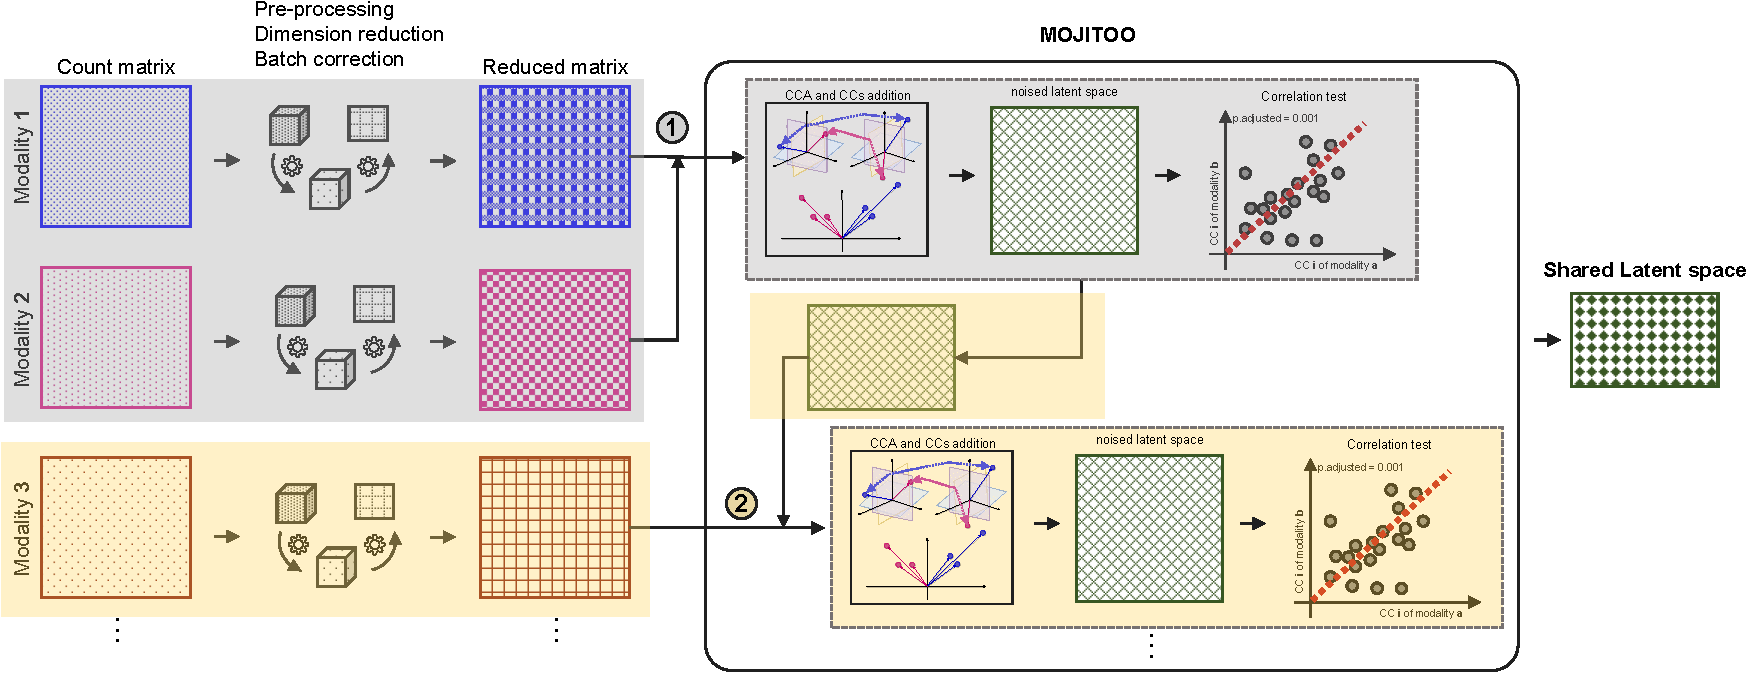
\includegraphics[width=0.95\textwidth]{MOJITOO_schematic/fig}
	\vspace{0.1cm}
	\caption[MOJITOO\_schematic.]{MOJITOO\_schematic}
	\label{fig:MOJITOO_schematic}
\end{figure}

\begin{table}[!ht]
	\centering
	\begin{tabular}{lll}
		\toprule
		\textbf{Package} & \textbf{Version} & \textbf{Website} \\
		\midrule
		  Rcpp  & >= 1.0.7& \url{} \\
		  Seurat & >= 3.2.3 & \url{} \\
		  Signac & >= 1.0.0& \url{} \\
		  reticulate & >= 1.22& \url{} \\
		  corpcor & >= 1.6.10 & \url{} \\
		  S4Vectors & >= 0.30.2 & \url{} \\
		  ramify & >= 0.3.3 & \url{} \\
		  plyr & >= 1.8.6 & \url{} \\
		  rhdf5 & >= 2.36.0 & \url{} \\
		  Matrix & >= 1.3-4 & \url{} \\
		  glue & >= 1.4.2 & \url{} \\
		  dplyr & >= 1.0.7 & \url{} \\
		  reshape2 & >= 1.4.4 & \url{} \\
		  pbapply & >= 1.5-0 & \url{} \\
		  ggplot2 & >= 3.3.5 & \url{} \\
		  ComplexHeatmap & >= 2.11.1 & \url{} \\
		  patchwork & >= 1.1.1 & \url{} \\
		  Gviz & >= Gviz & \url{} \\
		  grid & >= 4.1.0 & \url{} \\
		  tidyr & >= 1.1.4 & \url{} \\
		  fda & >= 5.5.1 & \url{} \\
		  assertthat & >= 0.2.1 & \url{} \\
		\bottomrule
	\end{tabular}
	\vspace{0.1cm}
	\caption[MOJITOO tool R package dependencies]{MOJITOO tool R package dependencies.}
	\label{tab:mojitoo_R_dependencies}
\end{table}
  

MOJITOO takes as input a set of matrices from $m$ modalities:
\begin{align}
    \mathcal{X}=\{X^{(1)},\cdots,X^{(m)}\}
\end{align}
where $X^{(i)} \in \mathbb{R}^{n\times s^{(i)}}$ represents the data of a particular single cell modality, $n$ represents the number of cells, and $s^{(i)}$ represents the number of features in modality $i$. Here, we focus on multimodal data, where the cells are the same across matrices and there is no direct relation between the features of the distinct modalities. 

\subsubsection{Reducing the dimension for each modality}

We first obtain a dimension reduced matrix for each modality independently using a modality-specific approach: 
\begin{align}
    Y^{(i)}=f^{(i)}(X^{(i)})
\end{align}
where $Y^{(i)} \in \mathbb{R}^{n\times p^{(i)}}$ represents the low-dimensional matrix for modality $i$, $p^{(i)}$ represents the number of dimensions and $f^{(i)}$ represents the specific dimension reduction method for this modality. MOJITOO uses latent semantic indexing (LSI) for scATAC-seq and principal component analysis (PCA) for other modalities, as is usual in the literature~\cite{granja2021archr, signac, hao2021integrated}.
The rationale behind the use of dimension reduction is two-fold. First, low-dimensional matrices reduce the computing time of the CCA analysis without impacting accuracy for a minimum number of dimensions. Moreover, it allows to work directly on batch-corrected data, which is usually represented in a low-dimensional space~\cite{hao2021integrated, korsunsky2019fast}. Of note, batch correction is recommended previous to MOJITOO, whenever the data is affected by batch effects. 

\subsubsection{Learning a shared space with canonical correlation analysis with two modalities}

MOJITOO aims to learn a shared latent space $Z$ from the set of low dimensional matrices   $\mathcal{Y}=\{Y^{(1)},\cdots,Y^{(m)}\}$
\begin{align}
    Z = \text{MOJITOO}(Y^{(1)}, \cdots, Y^{(m)}),
\end{align}
where $Z \in \mathbb{R}^{n\times k}$ represents the cells, $n$ is the number of cells and $k$ is the dimension of this latent space. When $\mathcal{Y}$ has two modalities, we first use CCA\footnote{This notation is based on a geometrical interpretation of CCA.} to project the matrices $Y^{(1)}$ and $Y^{(2)}$ to vectors ${\mathbf z_1^{(1)}}$ and ${\mathbf z_1^{(2)}}$:
\begin{equation}
\begin{split}
{\mathbf z_1^{(1)}}=Y^{(1)} {\mathbf w_1^{(1)}}, \\
{\mathbf z_1^{(2)}}=Y^{(2)} {\mathbf w_1^{(2)}},
\end{split}
\end{equation}
where ${\mathbf z_1^{(1)}}$ and ${\mathbf z_1^{(2)}}$ represent canonical components (CC). The vectors ${\mathbf w_1^{(1)}}$ and ${\mathbf w_1^{(2)}}$ can be obtained by solving the following optimization problem:
\begin{equation}
    \mathbf w_1^{(1)}, \mathbf w_1^{(2)} = \argmax \cos(\mathbf z_1^{(1)}, \mathbf z_1^{(2)}),
\end{equation}
where ${\mathbf w_1^{(1)}}\in\mathbb{R}^{p^{(1)}}$, ${\mathbf w_1^{(2)}}\in \mathbb{R}^{p^{(2)}}$ represent the first canonical weight vectors, and $\cos(\cdot)$ is the cosine similarity between two vectors $a$ and $b$ defined by:
\begin{equation}
    \cos(a,b)=\frac{a.b}{|a|.|b|}.
\end{equation}

This is repeated $\hat{k}=\min(p^{(1)}, p^{(2)})$ times, such that new canonical vectors are orthogonal to previously estimated vectors. These provide the matrices:
\begin{equation}
    \begin{split}
      W^{(1)} = \Big[ {\mathbf w}_1^{(1)},\cdots,{\mathbf w}_{\hat{k}}^{(1)}\Big], \\
      W^{(2)} = \Big[ {\mathbf w}_1^{(2)},\cdots,{\mathbf w}_{\hat{k}}^{(2)}\Big].
    \end{split}
\end{equation}
These can be used to estimate the modality transformed space as
\begin{equation}
    \begin{split}
      Z^{(1)}=Y^{(1)}\cdot W^{(1)}, \\
      Z^{(2)}=Y^{(2)}\cdot W^{(2)}.
    \end{split}
\end{equation}
A unique latent space is obtained as
\begin{align}
Z = Z^{(1)} + Z^{(2)},
\end{align}
where $Z\in\mathbb{R}^{n\times {k}}$ and ${k}$ is the number of canonical variables retained. 



\subsubsection{solving the problem of cannonical correlation analysis}

$\mathbf{X}_a\in \mathbb{R}^{n\times p}$

$\mathbf{X}_b\in \mathbb{R}^{n\times q}$

linear transformation: $\mathbf{X}_a{\mathbf w}_a={\mathbf z}_a$ and $\mathbf{X}_b{\mathbf w}_b={\mathbf z}_b$ 

objective:

$\cos \theta_1 = \underset{{\mathbf z}_a, {\mathbf z}_b \in\mathbb{R}^n}{\max}<{\mathbf z}_a, {\mathbf z}_b>$, subject to  $\|{\mathbf z}_a\|_2=1\quad \|{\mathbf z}_b\|_2=1$

$\qquad{\vdots}$

$\cos \theta_r = \underset{{\mathbf z}_a^r, {\mathbf z}_b^r \in\mathbb{R}^n}{\max}<{\mathbf z}_a^r, {\mathbf z}_b^r>$, subject to  $\|{\mathbf z}_a\|_2=1\quad \|{\mathbf z}_b\|_2=1$, $<{\mathbf z}_a^j, {\mathbf z}_a^r>=0\quad<{\mathbf z}_b^j, {\mathbf z}_b^r>=0$



empirical covariance matrix:  $C_{ab}=\frac{1}{n-1}\mathbf{X}_a^T\mathbf{X}_b$    Time complexity: $O(n\times p \times q)$

empirical variance matrix: $C_{aa}=\frac{1}{n-1}\mathbf{X}_a^T\mathbf{X}_a\quad C_{bb}=\frac{1}{n-1}\mathbf{X}_b^T\mathbf{X}_b$       Time complexity: $O(n\times p \times p)$,  $O(n\times q \times q)$

since correction between ${\mathbf z}_a$ and ${\mathbf z}_b$ does not change with the scaling, so that we can constrain ${\mathbf w}_a$ and ${\mathbf w}_b$:

$$
{\mathbf z}_a^T{\mathbf z}_a={\mathbf w}_a^T\mathbf{X}_a^T\mathbf{X}_a{\mathbf w}_a={\mathbf w}_a^T C_{aa}{\mathbf w}_a=1\\
{\mathbf z}_b^T{\mathbf z}_b={\mathbf w}_b^T\mathbf{X}_b^T\mathbf{X}_b{\mathbf w}_b={\mathbf w}_b^T C_{bb}{\mathbf w}_b=1
$$




since $\mathbf{X}_a$ and $\mathbf{X}_b$ should be centered, the covariance between  ${\mathbf z}_a$ and ${\mathbf z}_b$:

$$
{\mathbf z}_a^T{\mathbf z}_b={\mathbf w}_a^T\mathbf{X}_a^T\mathbf{X}_b{\mathbf w}_b={\mathbf w}_a^T C_{ab}{\mathbf w}_b
$$

$$
\cos \theta=\underset{{\mathbf z}_a, {\mathbf z}_b \in\mathbb{R}^n}{\max}<{\mathbf z}_a, {\mathbf z}_b>=\underset{{\mathbf w}_a\in \mathbb{R}^p, {\mathbf w}_b \in\mathbb{R}^q}{\max} {\mathbf w}_a^T C_{ab}{\mathbf w}_b\\
\textbf{ object to:  }  \|{\mathbf z}_a\|_2=\sqrt{{\mathbf w}_a^T C_{aa}{\mathbf w}_a}=1\quad \|{\mathbf z}_b\|_2=\sqrt{{\mathbf w}_b^T C_{bb}{\mathbf w}_b}=1
$$



Use Cholesky decomposition to decompose symmetric matrix 


$$
C_{aa}=C_{aa}^{1/2}C_{aa}^{1/2}
$$

$$
C_{bb}=C_{bb}^{1/2}C_{bb}^{1/2}
$$

$$
\begin{pmatrix}
C_{aa}^{-1/2} & {\mathbf 0}\\
{\mathbf 0} & C_{bb}^{-1/2}
\end{pmatrix}
\begin{pmatrix}
C_{aa} & C_{ab}\\
C_{ba} & C_{bb}
\end{pmatrix}
\begin{pmatrix}
C_{aa}^{-1/2} & {\mathbf 0}\\
{\mathbf 0} & C_{bb}^{-1/2}
\end{pmatrix}
=
\begin{pmatrix}
I_q & C_{aa}^{-1/2}C_{ab}C_{bb}^{-1/2}\\
C_{bb}^{-1/2}C_{ba}C_{aa}^{-1/2} & I_p
\end{pmatrix}
$$


$$
C_{aa}^{-1/2}C_{ab}C_{bb}^{-1/2}=U^TSV
$$

$$
\arg\max {\mathbf w}_a^T C_{ab}{\mathbf w}_b=\arg\max (C_{aa}^{1/2}{\mathbf w}_a)^TC_{aa}^{-1/2}C_{ab}C_{bb}^{-1/2}C_{bb}^{1/2}{\mathbf w}_b
$$


$$
{\mathbf w}_a = C_{aa}^{-1/2}U\quad {\mathbf w}_b = C_{bb}^{-1/2}V\quad
$$

$C_{aa}^{-1/2}C_{ab}C_{bb}^{-1/2}$ SVD fit the constraint:

Let $\tilde{{\mathbf w}}_a=C_{aa}^{1/2}{\mathbf w}_a$ and  $\tilde{{\mathbf w}}_b=C_{bb}^{1/2}{\mathbf w}_b$ , we can write the constraint ${\mathbf w}_a^T C_{aa}{\mathbf w}_a={\mathbf w}_b^T C_{bb}{\mathbf w}_b=1$ as:
$$
\tilde{{\mathbf w}}_a^T\tilde{{\mathbf w}}_a=1\\
\tilde{{\mathbf w}}_b^T\tilde{{\mathbf w}}_b=1
$$
Since $C_{aa}$ and $C_{bb}$ are non-singular, $C_{aa}^{1/2}$ and $C_{bb}^{1/2}$ are non-singular, the objective (3)
$$
\arg\max \tilde{{\mathbf w}}_a C_{aa}^{-1/2}C_{ab}C_{bb}^{-1/2}\tilde{{\mathbf w}}_b\\
\textbf{subject to } \|\tilde{\mathbf w}_a\|=1\textbf{ and  }\|\tilde{\mathbf w}_b\|=1
$$

$$
\tilde{\mathbf w}_a=u_1\\
\tilde{\mathbf w}_b=v_1
$$

$$
{\mathbf w}_{a_1}=C_{aa}^{-1/2}u_1\\
{\mathbf w}_{b_1}=C_{bb}^{-1/2}v_1
$$




SVD solving

$$
A=U^TSV, \textbf{where } U^T=U^{-1}, V^T=V^{-1}, S\textbf{ is diagnal}
$$


$$
AA^T=USV^TVS^TU^T=US^2U^T\\
A^TA=VS^TU^TUSV^T=VS^2V^T
$$

$$
\lambda_i=\sigma_i^2\\
AA^Tu_i = \lambda_i u_i\\
A^TAv_i = \lambda_i v_i
$$

$$
\textbf{Time complexity: }O(\min(p^2q,qp^2))
$$





To further remove the noise from the latent space $Z$, we only keep highly correlated canonical components $z_i^{(1)}$ and $z_i^{(2)}$ by measuring the Pearson correlation and using a student's $t$-test for significance. The $p$-values are then corrected using BH(Benjamini Hochberg)\cite{benjamini1995controlling} and only canonical components with adjusted p-values < 0.05 are retained. 

MOJITOO uses an algorithm based on generalized eigenvector decomposition~\cite{Ramsay97functionaldata} to estimate the canonical components. MOJITOO has a time complexity of $\mathcal{O}(max\{p^{(1)},p^{(2)}\}^{2} \times n)$ for computing covariance matrices and $\mathcal{O}(\min\{p^{(1)},p^{(2)}\}\times p^{(1)}\times p^{(2)})$ for the eigenvector decomposition. As $n$ (number of cells) is usually 100 times larger than $p^{(i)}$ (number of reduced dimensions in $Y^{(i)}$) the first term dominates the complexity. 

Of note, CCA is one of the several steps in the integration algorithm of an earlier version of Seurat~\cite{butler2018integrating}. This had the objective to integrate distinct scRNA-seq experiments and CCA was performed in the common gene space, i.e. on transposed $Y^{(i)}$ matrices and the objective was to find matching cells.

\subsubsection{Learning a shared space for multiple modalities}

For the case that $\mathcal{Y}$ has more than two modalities, we perform the pairwise integration of modalities starting with the pair with highest dimensionality. The result of this CCA is then used for integration with the next modality. See algorithm~\ref{alg:MOJITOO} for a brief description, which receives a set of matrices $\{Y^{(1)},\cdots, Y^{(m)}\}$ with increasing dimensions $p^{(i)}\geq p^{(i+1)}$ as input. This heuristic algorithm was adopted to avoid the high computational costs of multiple CCA, which grows exponentially with the number of modalities. 
\begin{algorithm}
	\Input{
	$Y^{(1)},...,Y^{(m)}$
	}

	$i \gets 2$ \\
	$Z^{(1)} \gets Y^{(1)}$ \\
	\While{$i < m$}
	{
		$W^{(1)}, W^{(2)} \gets CCA(Z^{(1)}, Y^{(i)})$ \\ 
		$Z^{(1)} \gets Z^{(1)}\times W^{(1)}$ \\ 
		$Z^{(2)} \gets Y^{(i)}\times W^{(2)}$  \\
		$Z \gets Z^{(1)} + Z^{(2)}$ \\ 
		$Z \gets Z[, 1:k]$\Comment{only consider significantly correlated dimension } 
		$Z^{(1)} \gets Z$ \\
		$i \gets i+1$  \\
	}
	\Return $\mathbf{Z}$ 
	\caption{Multimodal MOJITOO Algorithm }
	\label{alg:MOJITOO}
\end{algorithm}

\subsection{Discussion}

\section{Single cell trajectory inference}
\label{methods:TI}

%a table shows the R dependencies
\subsubsection{trajectory inference}
\begin{figure}[!ht]
	\centering
	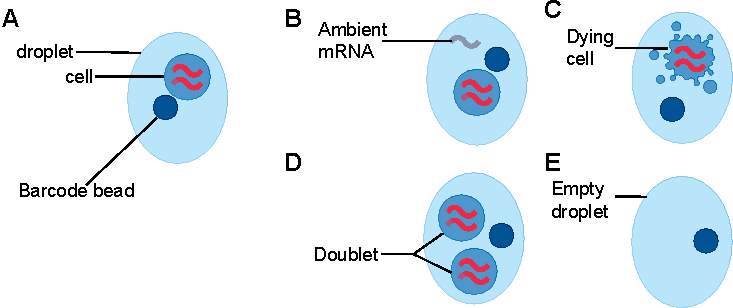
\includegraphics[width=0.95\textwidth]{PHLOWER_schematic/fig}
	\vspace{0.1cm}
	\caption[PHLOWER\_schematic.]{PHLOWER\_schematic}
	\label{fig:PHLOWER_schematic}
\end{figure}

% python package dependencies
\begin{table}[!ht]
	\centering
	\begin{tabular}{lll}
		\toprule
		\textbf{Package} & \textbf{Version} & \textbf{Website} \\
		\midrule
			numpy& >=1.23.5 & \url{https://numpy.org/} \\
			matplotlib& >=3.6.0 & \url{https://matplotlib.org/} \\
			seaborn& >=0.12.0 & \url{https://seaborn.pydata.org/} \\
			pydot& >=1.4.2 & \url{https://github.com/pydot/pydot} \\
			igraph& >=0.10.5 & \url{https://igraph.org/python/} \\
			scikit-learn& >=1.1.2 & \url{https://scikit-learn.org/stable/} \\
			scipy& >=1.10.1 & \url{https://www.scipy.org/} \\
			pandas& >=1.3.5 & \url{https://pandas.pydata.org/} \\
			plotly& >=5.13.1 & \url{https://plotly.com/} \\
			tqdm& >=4.64.1 & \url{https://github.com/tqdm/tqdm} \\
			leidenalg& >=0.9.1 & \url{https://github.com/vtraag/leidenalg} \\
			%louvain& >=0.8.0 & \url{} \\
			colorcet& >=3.0.1 & \url{https://github.com/holoviz/colorcet} \\
			umap-learn& >=0.5.3 & \url{https://github.com/lmcinnes/umap} \\
			scikit-sparse& >=0.4.8 & \url{https://github.com/scikit-sparse/scikit-sparse} \\
			scanpy& >=1.9.3 & \url{https://github.com/scverse/scanpy} \\
			anndata& >=0.8.0 & \url{https://github.com/scverse/anndata} \\
		\bottomrule
	\end{tabular}
	\vspace{0.1cm}
	\caption[PHLOWER tool python package dependencies]{PHLOWER tool python package dependencies.}
	\label{tab:phlower_python_dependencies}
\end{table}
% a table shows the python dependencies
% check how to rotate the title text of a table, see Li's table 3.2
\subsection{Discussion}
